\chapter*{附录A}
\markboth{附录A}{附录A} % 设置页眉显示内容
\addcontentsline{toc}{chapter}{附录A}

% PDF有多页,需要循环插入每一页
% 可以使用下面的代码循环插入所有页面
\newcounter{pdftotalpages}
\newcounter{pdfpage}
\setcounter{pdftotalpages}{12} % 设置PDF的总页数
\setcounter{pdfpage}{2}
{\centering
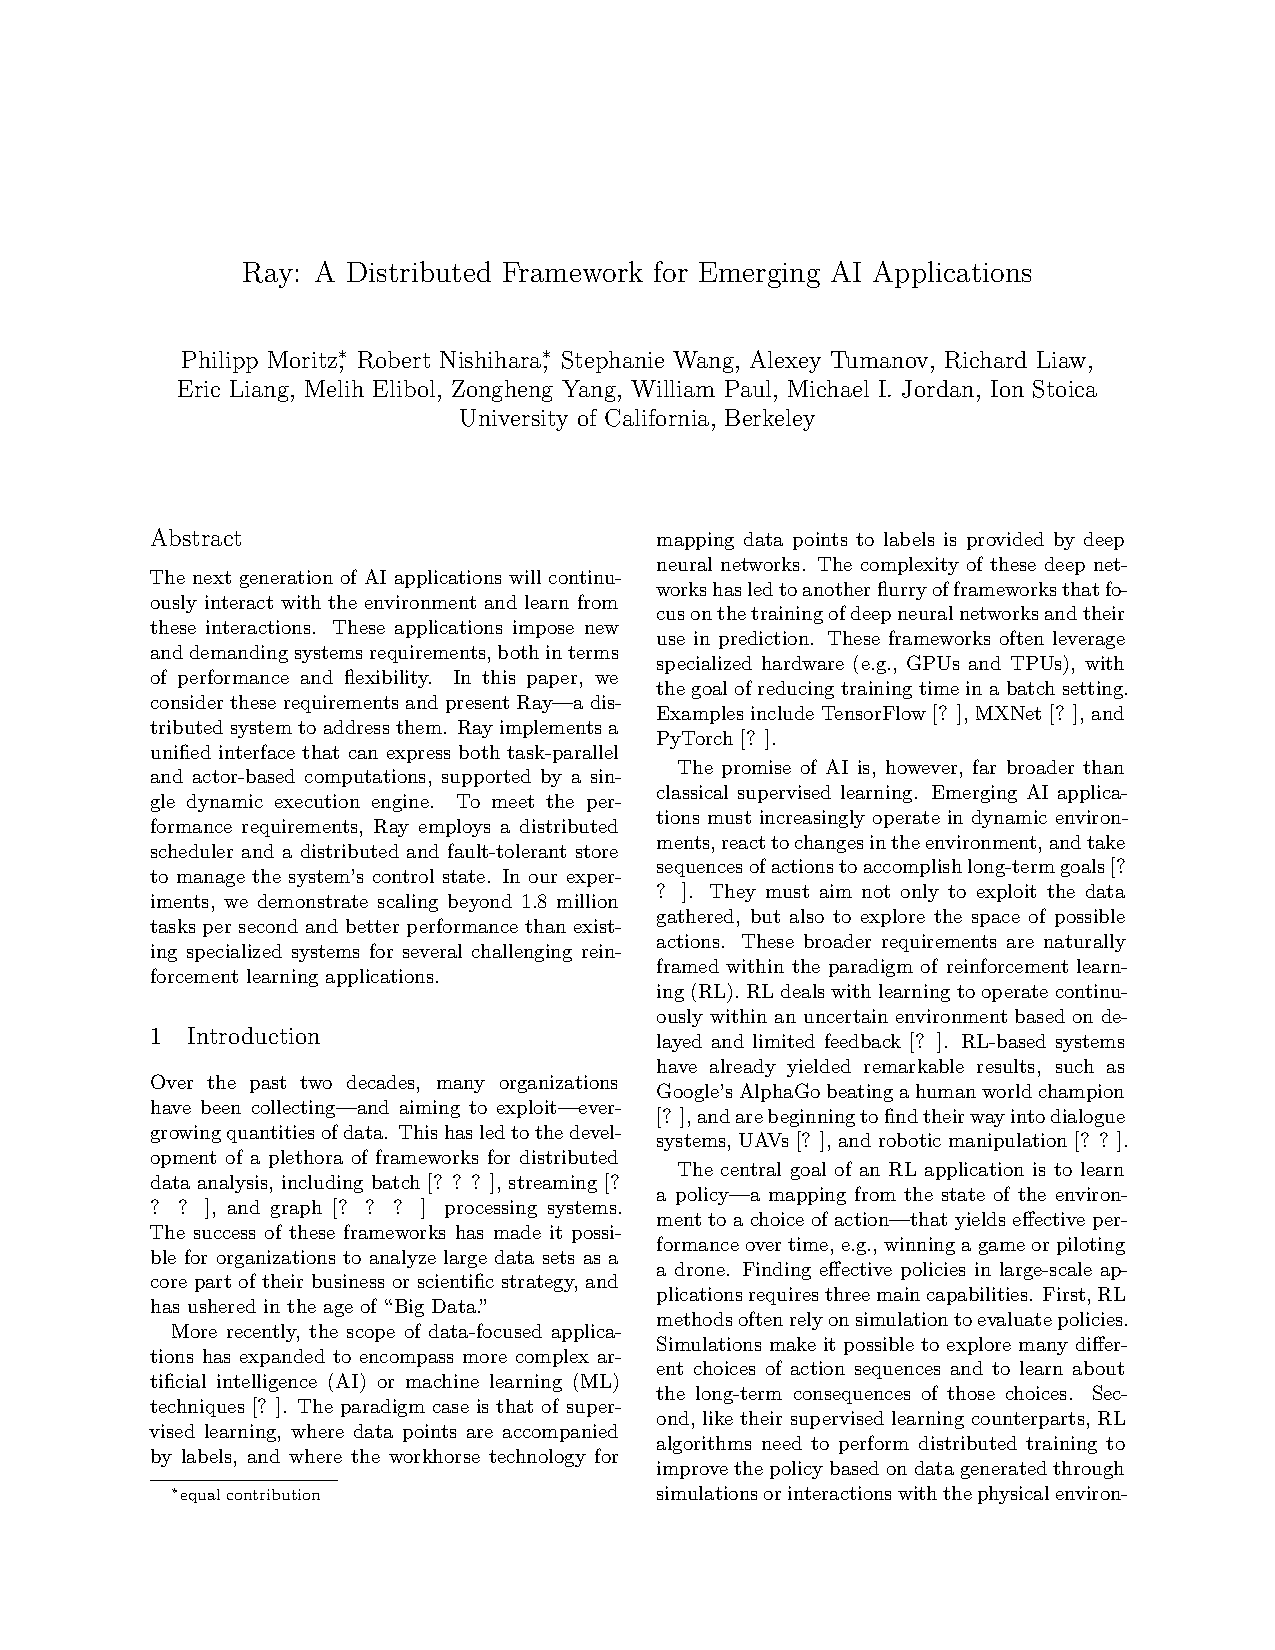
\includegraphics[width=\textwidth, page=1, trim = 20mm 40mm 20mm 30mm]{pdfs/ray.pdf}
\whiledo{\value{pdfpage} < \value{pdftotalpages}}{%
  \stepcounter{pdfpage}
  \clearpage
  \includegraphics[width=\textwidth,page=\thepdfpage,trim = 25mm 40mm 25mm 25mm]{pdfs/ray.pdf}
}
}

\chapter*{附录B}
\markboth{附录B}{附录B} % 设置页眉显示内容
\addcontentsline{toc}{chapter}{附录B}

% PDF有多页,需要循环插入每一页
% 可以使用下面的代码循环插入所有页面
\setcounter{pdftotalpages}{7} % 设置PDF的总页数
\setcounter{pdfpage}{2}
{\centering

\includegraphics[width=\textwidth, page=1, trim = 20mm 40mm 20mm 30mm]{pdfs/translation.pdf}
\whiledo{\value{pdfpage} < \value{pdftotalpages}}{%
  \stepcounter{pdfpage}
  \clearpage
  
\includegraphics[width=\textwidth,page=\thepdfpage,trim = 25mm 40mm 25mm 25mm]{pdfs/translation.pdf}
}
}

%控制为偶数页结束
\newpage
\null